%===============================================================================
% LaTeX sjabloon voor de bachelorproef toegepaste informatica aan HOGENT
% Meer info op https://github.com/HoGentTIN/latex-hogent-report
%===============================================================================

\documentclass[dutch,dit,thesis]{hogentreport}

% TODO:
% - If necessary, replace the option `dit`' with your own department!
%   Valid entries are dbo, dbt, dgz, dit, dlo, dog, dsa, soa
% - If you write your thesis in English (remark: only possible after getting
%   explicit approval!), remove the option "dutch," or replace with "english".

\usepackage{lipsum} % For blind text, can be removed after adding actual content
\usepackage{xcolor, soul}

%% Pictures to include in the text can be put in the graphics/ folder
\graphicspath{{../graphics/}}

%% For source code highlighting, requires pygments to be installed
%% Compile with the -shell-escape flag!
%\usepackage[chapter]{minted}
%% If you compile with the make_thesis.{bat,sh} script, use the following
%% import instead:
\usepackage[chapter,outputdir=../output]{minted}
\usemintedstyle{solarized-light}

%% Formatting for minted environments.
\setminted{%
    autogobble,
    frame=lines,
    breaklines,
    linenos,
    tabsize=4
}

%% Ensure the list of listings is in the table of contents
\renewcommand\listoflistingscaption{%
    \IfLanguageName{dutch}{Lijst van codefragmenten}{List of listings}
}
\renewcommand\listingscaption{%
    \IfLanguageName{dutch}{Codefragment}{Listing}
}
\renewcommand*\listoflistings{%
    \cleardoublepage\phantomsection\addcontentsline{toc}{chapter}{\listoflistingscaption}%
    \listof{listing}{\listoflistingscaption}%
}

% Other packages not already included can be imported here

%%---------- Document metadata -------------------------------------------------
% TODO: Replace this with your own information
\author{Lisa Verhoeyen}
\supervisor{Mevr. V. Depestele}
\cosupervisor{Dhr. J. Campens}
\title[Optionele ondertitel]%
    {Titel van de bachelorproef}
\academicyear{\advance\year by -1 \the\year--\advance\year by 1 \the\year}
\examperiod{1}
\degreesought{\IfLanguageName{dutch}{Professionele bachelor in de toegepaste informatica}{Bachelor of applied computer science}}
\partialthesis{false} %% To display 'in partial fulfilment'
%\institution{Internshipcompany BVBA.}

%% Add global exceptions to the hyphenation here
\hyphenation{back-slash}

%% The bibliography (style and settings are  found in hogentthesis.cls)
\usepackage[backend=biber,style=apa]{biblatex}
\DeclareLanguageMapping{dutch}{dutch-apa}
\addbibresource{bachproef.bib}            %% Bibliography file
\addbibresource{../voorstel/voorstel.bib} %% Bibliography research proposal
\defbibheading{bibempty}{}

%% Prevent empty pages for right-handed chapter starts in twoside mode
\renewcommand{\cleardoublepage}{\clearpage}

\renewcommand{\arraystretch}{1.2}

%% Content starts here.
\begin{document}

%---------- Front matter -------------------------------------------------------

\frontmatter

\hypersetup{pageanchor=false} %% Disable page numbering references
%% Render a Dutch outer title page if the main language is English
\IfLanguageName{english}{%
    %% If necessary, information can be changed here
    \degreesought{Professionele Bachelor toegepaste informatica}%
    \begin{otherlanguage}{dutch}%
       \maketitle%
    \end{otherlanguage}%
}{}

%% Generates title page content
\maketitle
\hypersetup{pageanchor=true}

%%=============================================================================
%% Voorwoord
%%=============================================================================

\chapter*{\IfLanguageName{dutch}{Woord vooraf}{Preface}}%
\label{ch:voorwoord}

%% TODO:
%% Het voorwoord is het enige deel van de bachelorproef waar je vanuit je
%% eigen standpunt (``ik-vorm'') mag schrijven. Je kan hier bv. motiveren
%% waarom jij het onderwerp wil bespreken.
%% Vergeet ook niet te bedanken wie je geholpen/gesteund/... heeft

Voor mijn bachelorproef wou ik graag iets doen dat een uitdaging was, maar dat ook verder nog nuttig zou zijn na het afronden van mijn bachelorproef, wat met dit onderwerp zeker bereikt werd. Ondanks het feit dat het trainen niet het resultaat leverde waarop ik gehoopt had, heb ik wel veel bijgeleerd en ben ervan overtuigd dat als hier nog verder op gewerkt wordt, dit nog steeds een nuttig onderzoek was.

Ik wil in de eerste plaats mijn co-promotor dhr. Jorrit Campens bedanken voor het aanreiken van dit onderwerp en de begeleiding tijdens het verloop van de bachelorproef. Het was een unieke kans om iets bij te leren en ondertussen te werken aan iets dat een effect zou kunnen hebben in de opleiding voor toekomstige verpleegkundigen.

Ook wil ik graag mijn promotor mevr. Veerle Depestele bedanken voor de opvolgingen tijdens mijn onderzoek en het geven van feedback waar nodig. Ik ben ervan overtuigd dat dit geholpen heeft om deze bachelorproef tot een goed einde te brengen.

Tenslotte wil ik ook mijn familie en vrienden bedanken die mij gesteund hebben doorheen deze bachelorproef, maar ook gedurende de opleiding die mij tot deze bachelorproef geleid heeft.
%%=============================================================================
%% Samenvatting
%%=============================================================================

% TODO: De "abstract" of samenvatting is een kernachtige (~ 1 blz. voor een
% thesis) synthese van het document.
%
% Een goede abstract biedt een kernachtig antwoord op volgende vragen:
%
% 1. Waarover gaat de bachelorproef?
% 2. Waarom heb je er over geschreven?
% 3. Hoe heb je het onderzoek uitgevoerd?
% 4. Wat waren de resultaten? Wat blijkt uit je onderzoek?
% 5. Wat betekenen je resultaten? Wat is de relevantie voor het werkveld?
%
% Daarom bestaat een abstract uit volgende componenten:
%
% - inleiding + kaderen thema
% - probleemstelling
% - (centrale) onderzoeksvraag
% - onderzoeksdoelstelling
% - methodologie
% - resultaten (beperk tot de belangrijkste, relevant voor de onderzoeksvraag)
% - conclusies, aanbevelingen, beperkingen
%
% LET OP! Een samenvatting is GEEN voorwoord!

%%---------- Nederlandse samenvatting -----------------------------------------
%
% TODO: Als je je bachelorproef in het Engels schrijft, moet je eerst een
% Nederlandse samenvatting invoegen. Haal daarvoor onderstaande code uit
% commentaar.
% Wie zijn bachelorproef in het Nederlands schrijft, kan dit negeren, de inhoud
% wordt niet in het document ingevoegd.

\IfLanguageName{english}{%
\selectlanguage{dutch}
\chapter*{Samenvatting}
\lipsum[1-4]
\selectlanguage{english}
}{}

%%---------- Samenvatting -----------------------------------------------------
% De samenvatting in de hoofdtaal van het document

\chapter*{\IfLanguageName{dutch}{Samenvatting}{Abstract}}

Ondanks het feit dat de zorgsector de dag van vandaag vooral op persoonsgerichte zorgverlening focust, ervaren oudere patiënten vaak dat de communicatie te betuttelend is. Dit fenomeen staat bekend als elderspeak of secondary babytalk. Om dit tegen te gaan is er vanuit de opleiding verpleegkunde aan HOGENT het initiatief genomen om een applicatie te gebruiken die de studenten erop wijst dat ze gebruik maken van elderspeak. Deze applicatie werd reeds ontworpen in voorgaande bachelorproeven aan HOGENT, maar er ontbreken nog een aantal functionaliteiten voordat deze gebruikt kan worden in de opleiding.

Deze bachelorproef heeft als doel een model te trainen dat stemmen kan onderscheiden en dit te implementeren in de applicatie zodat de optie bestaat om enkel de stem van de zorgverlener te analyseren op signalen van secondary babytalk. Hiervoor werd eerst onderzoek gedaan naar bestaande modellen, waarna deze modellen getest werden op bruikbaarheid voor deze bachelorproef. Na deze testen werd gekozen om verder te gaan met pyannote-audio. Dit model werd verder getraind met Vlaamse audio.

Na het trainingsproces moest geconcludeerd worden dat de resultaten van het trainen nog niet accuraat genoeg zijn en er dus geen implementatie in de applicatie kon gebeuren. Dit leidde wel tot enkele mogelijkheden voor verder onderzoek. Het gebruik van een ruisfilter, trainen op meer data of trainen op twee verschillende databanken zouden kunnen leiden tot een beter resultaat, waarna implementatie in de applicatie kan gebeuren.



%---------- Inhoud, lijst figuren, ... -----------------------------------------

\tableofcontents

% In a list of figures, the complete caption will be included. To prevent this,
% ALWAYS add a short description in the caption!
%
%  \caption[short description]{elaborate description}
%
% If you do, only the short description will be used in the list of figures

\listoffigures

% If you included tables and/or source code listings, uncomment the appropriate
% lines.
\listoftables

\listoflistings

% Als je een lijst van afkortingen of termen wil toevoegen, dan hoort die
% hier thuis. Gebruik bijvoorbeeld de ``glossaries'' package.
% https://www.overleaf.com/learn/latex/Glossaries

%---------- Kern ---------------------------------------------------------------

\mainmatter{}

% De eerste hoofdstukken van een bachelorproef zijn meestal een inleiding op
% het onderwerp, literatuurstudie en verantwoording methodologie.
% Aarzel niet om een meer beschrijvende titel aan deze hoofdstukken te geven of
% om bijvoorbeeld de inleiding en/of stand van zaken over meerdere hoofdstukken
% te verspreiden!

%%=============================================================================
%% Inleiding
%%=============================================================================

\chapter{\IfLanguageName{dutch}{Inleiding}{Introduction}}%
\label{ch:inleiding}

De dag van vandaag focust de zorg- en welzijnssector vooral op persoonsgerichte zorgverlening. Dit impliceert dat de zorgverleners hun communicatiestijl aanpassen aan de zorgvragers. In de context van zorgverlening bij ouderen wordt de communicatiestijl echter vaak als te betuttelend ervaren. Men noemt dit fenomeen secondary babytalk of elderspeak. Om dit tegen te gaan, wil de opleiding verpleegkunde aan HOGENT gebruik maken van een applicatie die zou helpen om via speech-to-text de secondary babytalk op te sporen. Aan de hand daarvan zouden ze dan feedback kunnen geven aan de studenten tijdens praktijksessies in het Zorglab.

Het Zorglab is een lokaal dat voornamelijk gebruikt wordt tijdens de praktijklessen in de opleiding verpleegkunde. Het lokaal bestaat uit 2 ruimtes waarin camera's hangen. De studenten kunnen hier microfoons dragen zodat medestudenten in een derde ruimte kunnen volgen wat er gebeurt en ondertussen feedback krijgen van de lector. Hier zou dus gebruik gemaakt worden van de applicatie om snel de voorvallen van elderspeak op te sommen zodat de studenten ook feedback kunnen krijgen op wat ze zelf gedaan hebben en niet enkel op wat studenten in een andere groep doen.

\section{\IfLanguageName{dutch}{Probleemstelling}{Problem Statement}}%
\label{sec:probleemstelling}

In voorgaande jaren werd in de bachelorproeven van \textcite{Govaerts2022}, \textcite{Gussem2022} en \textcite{Daems2023} reeds succesvol een applicatie ontwikkeld die signalen van elderspeak kan herkennen aan de hand van kenmerken zoals toonhoogte en stemvolume. In deze applicatie kan men een audiofragment uploaden en dit aan de hand van een aantal parameters laten analyseren. In de jaren die daarop volgden werd er in de bachelorproeven van \textcite{Branden2024}, \textcite{Coetsiers2024} en \textcite{Schryver2024} onderzoek gedaan naar het integreren van een model dat spraak kan omzetten naar tekst, maar hier werd aangetoond dat de accuraatheid van bestaande modellen onvoldoende blijkt te zijn om een kwaliteitsvolle transcriptie uit te voeren van gesproken Nederlands.

Aangezien de implementatie van speech-to-text nog niet geslaagd was, was er vraag naar een methode om stemmen te onderscheiden. 
Enerzijds werd deze vraag gesteld met als doel de implementatie van transcriptie voor Vlaamse audio te vereenvoudigen. Anderzijds heeft het als doel ook gebruikt te worden om er in de applicatie voor te zorgen dat enkel de stem van de student geanalyseerd wordt op signalen van elderspeak.

\section{\IfLanguageName{dutch}{Onderzoeksvraag}{Research question}}%
\label{sec:onderzoeksvraag}

Concreet wordt er voor deze bachelorproef de volgende onderzoeksvraag gesteld: hoe kan ervoor gezorgd worden dat de applicatie onderscheid maakt tussen de stem van de zorgverlener en die van de zorgvrager? Dit kan opgesplitst worden in verschillende deelvragen:
\begin{itemize}
	\item Wat zijn reeds bestaande modellen en python libraries die stemmen kunnen herkennen en onderscheiden?
	\item Is het mogelijk om de reeds bestaande modellen (die meestal op Engelstalige audio getraind zijn) te trainen om Vlaamse sprekers te kunnen onderscheiden?
	\item Wat zijn de beste parameters om een model te trainen op het onderscheiden en afzonderen van stemmen?
	\item Is het mogelijk om het getrainde model in de applicatie te integreren?
\end{itemize} 

\section{\IfLanguageName{dutch}{Onderzoeksdoelstelling}{Research objective}}%
\label{sec:onderzoeksdoelstelling}

Het beoogde resultaat van deze bachelorproef bestaat uit twee delen. Het eerste deel is een getraind model dat succesvol stemmen in audiofragmenten met Vlaamstalige sprekers kan onderscheiden.\\
Het tweede deel is een succesvolle integratie van dit model in de applicatie van het Zorglab zodat deze de functionaliteit heeft om stemmen te onderscheiden en dit model eventueel gebruikt kan worden voor verdere toepassingen rond speech-to-text in de applicatie.

\section{\IfLanguageName{dutch}{Opzet van deze bachelorproef}{Structure of this bachelor thesis}}%
\label{sec:opzet-bachelorproef}

% Het is gebruikelijk aan het einde van de inleiding een overzicht te
% geven van de opbouw van de rest van de tekst. Deze sectie bevat al een aanzet
% die je kan aanvullen/aanpassen in functie van je eigen tekst.

De rest van deze bachelorproef is als volgt opgebouwd:

In Hoofdstuk~\ref{ch:stand-van-zaken} wordt een overzicht gegeven van de stand van zaken op basis van een literatuurstudie. Dit houdt in dat er wordt besproken wat de applicatie al kan en wat er op dit moment al mogelijk is als het gaat over onderscheiden van stemmen.

In Hoofdstuk~\ref{ch:methodologie} wordt de methodologie toegelicht en worden de gebruikte onderzoekstechnieken besproken om een antwoord te kunnen formuleren op de onderzoeksvragen.

% TODO: Vul hier aan voor je eigen hoofstukken, één of twee zinnen per hoofdstuk

In Hoofdstuk~\ref{ch:conclusie}, tenslotte, wordt de conclusie gegeven en een antwoord geformuleerd op de onderzoeksvragen. Daarbij wordt ook een aanzet gegeven voor toekomstig onderzoek binnen dit domein.
\chapter{\IfLanguageName{dutch}{Stand van zaken}{State of the art}}%
\label{ch:stand-van-zaken}

% Tip: Begin elk hoofdstuk met een paragraaf inleiding die beschrijft hoe
% dit hoofdstuk past binnen het geheel van de bachelorproef. Geef in het
% bijzonder aan wat de link is met het vorige en volgende hoofdstuk.

% Pas na deze inleidende paragraaf komt de eerste sectiehoofding.

Dit hoofdstuk bevat je literatuurstudie. De inhoud gaat verder op de inleiding, maar zal het onderwerp van de bachelorproef *diepgaand* uitspitten. De bedoeling is dat de lezer na lezing van dit hoofdstuk helemaal op de hoogte is van de huidige stand van zaken (state-of-the-art) in het onderzoeksdomein. Iemand die niet vertrouwd is met het onderwerp, weet nu voldoende om de rest van het verhaal te kunnen volgen, zonder dat die er nog andere informatie moet over opzoeken \autocite{Pollefliet2011}.

Je verwijst bij elke bewering die je doet, vakterm die je introduceert, enz.\ naar je bronnen. In \LaTeX{} kan dat met het commando \texttt{$\backslash${textcite\{\}}} of \texttt{$\backslash${autocite\{\}}}. Als argument van het commando geef je de ``sleutel'' van een ``record'' in een bibliografische databank in het Bib\LaTeX{}-formaat (een tekstbestand). Als je expliciet naar de auteur verwijst in de zin (narratieve referentie), gebruik je \texttt{$\backslash${}textcite\{\}}. Soms is de auteursnaam niet expliciet een onderdeel van de zin, dan gebruik je \texttt{$\backslash${}autocite\{\}} (referentie tussen haakjes). Dit gebruik je bv.~bij een citaat, of om in het bijschrift van een overgenomen afbeelding, broncode, tabel, enz. te verwijzen naar de bron. In de volgende paragraaf een voorbeeld van elk.

\textcite{Knuth1998} schreef een van de standaardwerken over sorteer- en zoekalgoritmen. Experten zijn het erover eens dat cloud computing een interessante opportuniteit vormen, zowel voor gebruikers als voor dienstverleners op vlak van informatietechnologie~\autocite{Creeger2009}.

Let er ook op: het \texttt{cite}-commando voor de punt, dus binnen de zin. Je verwijst meteen naar een bron in de eerste zin die erop gebaseerd is, dus niet pas op het einde van een paragraaf.

\begin{figure}
  \centering
  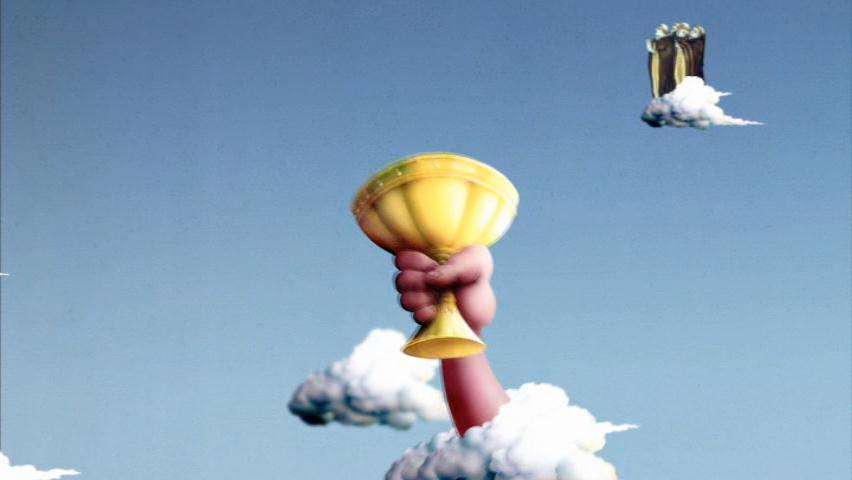
\includegraphics[width=0.8\textwidth]{grail.jpg}
  \caption[Voorbeeld figuur.]{\label{fig:grail}Voorbeeld van invoegen van een figuur. Zorg altijd voor een uitgebreid bijschrift dat de figuur volledig beschrijft zonder in de tekst te moeten gaan zoeken. Vergeet ook je bronvermelding niet!}
\end{figure}

\begin{listing}
  \begin{minted}{python}
    import pandas as pd
    import seaborn as sns

    penguins = sns.load_dataset('penguins')
    sns.relplot(data=penguins, x="flipper_length_mm", y="bill_length_mm", hue="species")
  \end{minted}
  \caption[Voorbeeld codefragment]{Voorbeeld van het invoegen van een codefragment.}
\end{listing}

\lipsum[7-20]

\begin{table}
  \centering
  \begin{tabular}{lcr}
    \toprule
    \textbf{Kolom 1} & \textbf{Kolom 2} & \textbf{Kolom 3} \\
    $\alpha$         & $\beta$          & $\gamma$         \\
    \midrule
    A                & 10.230           & a                \\
    B                & 45.678           & b                \\
    C                & 99.987           & c                \\
    \bottomrule
  \end{tabular}
  \caption[Voorbeeld tabel]{\label{tab:example}Voorbeeld van een tabel.}
\end{table}


%%=============================================================================
%% Methodologie
%%=============================================================================

\chapter{\IfLanguageName{dutch}{Methodologie}{Methodology}}%
\label{ch:methodologie}

%% TODO: In dit hoofstuk geef je een korte toelichting over hoe je te werk bent
%% gegaan. Verdeel je onderzoek in grote fasen, en licht in elke fase toe wat
%% de doelstelling was, welke deliverables daar uit gekomen zijn, en welke
%% onderzoeksmethoden je daarbij toegepast hebt. Verantwoord waarom je
%% op deze manier te werk gegaan bent.
%% 
%% Voorbeelden van zulke fasen zijn: literatuurstudie, opstellen van een
%% requirements-analyse, opstellen long-list (bij vergelijkende studie),
%% selectie van geschikte tools (bij vergelijkende studie, "short-list"),
%% opzetten testopstelling/PoC, uitvoeren testen en verzamelen
%% van resultaten, analyse van resultaten, ...
%%
%% !!!!! LET OP !!!!!
%%
%% Het is uitdrukkelijk NIET de bedoeling dat je het grootste deel van de corpus
%% van je bachelorproef in dit hoofstuk verwerkt! Dit hoofdstuk is eerder een
%% kort overzicht van je plan van aanpak.
%%
%% Maak voor elke fase (behalve het literatuuronderzoek) een NIEUW HOOFDSTUK aan
%% en geef het een gepaste titel.

Dit hoofdstuk bespreekt kort de fasen van het onderzoek. Per fase word kort besproken wat de doelstelling is en welke keuzes gemaakt werden. In figuur \ref{fig:flow-chart} wordt een overzicht getoond van de verschillende fasen en hoe deze elkaar opvolgen.

\paragraph{Literatuurstudie en modellen zoeken}
Deze fase bestaat uit het opzoeken van info omtrent diarization en welke bestaande modellen hier al voor zijn. Hieruit worden de modellen gekozen die het meeste potentieel lijken te hebben om tot een goed eindresultaat te komen en wordt gekeken wat de beste manier van aanpakken is.\\
Naast het zoeken naar modellen, wordt ook gezocht naar methoden om deze modellen te evalueren. Dit zorgt ervoor dat er een gegronde keuze kan gemaakt worden om verder te gaan met een specifiek model. Dit zorgt er in een latere fase ook voor dat er gekozen kan worden voor de beste parameters voor het model.

\paragraph{Modellen testen}
Tijdens deze fase wordt getest hoe bruikbaar de gevonden modellen effectief zijn en wat het beste model is om mee verder te gaan. Dit wordt gedaan door eerst te kijken naar het gemak om het model te installeren en lokaal werkend te krijgen. Hierna wordt een audiofragment gegeven aan de modellen en wordt gekeken naar de accuraatheid waarmee elk model de stemmen in dit fragment al kan onderscheiden. Uiteindelijk wordt er ook gekeken naar de mogelijkheid om het model verder te trainen om een beter resultaat te kunnen bekomen. Op basis van deze criteria wordt dan gekozen met welk model verder gegaan wordt in de volgende fasen.

\paragraph{Voorbereiden van de trainingsdata}
In deze fase wordt gezocht naar bruikbare Vlaamse audiofragmenten. Voornamelijk wordt gezocht naar Vlaamse televisieprogramma's en podcasts op \url{hetarchief.be} en YouTube. Op basis van de gevonden audio worden dan RTTM- en UEM-bestanden geschreven en afhankelijk van het gekozen model op de juiste manier opgeslagen. RTTM (Rich Transcription Time Marked) is een tekstgebaseerd bestandstype die bestaat uit tijdsmarkeringen die aangeven wanneer een woord of zin start en eindigt en die voornamelijk gebruikt wordt in spraak herkennende software \autocite{filext}. UEM (Un-partitioned Evaluation Map) bestanden worden gebruikt om aan te duiden welke delen van de audiobestanden gebruikt zijn om de RTTM-bestanden op te stellen \autocite{Ryant}.

\paragraph{Model trainen en finetunen}
Tijdens deze fase wordt het gekozen model getraind aan de hand van de data uit de vorige fase. Voor en na het trainen wordt het model geëvalueerd, aan de hand van methoden die in de eerste fase gevonden werden, om te kijken of het trainen het model accurater maakt dan het was voor het trainen. Hierna zullen de parameters van het model verder gefinetuned worden, waarna de accuraatheid opnieuw geëvalueerd wordt en eventueel meer finetuning plaatsvindt, tot een zo accuraat mogelijk model bekomen wordt.

\paragraph{Implementatie in de applicatie}
In deze laatste fase zal het model opgeslagen worden en geïmplementeerd worden in de broncode van de reeds bestaande applicatie. Er zal ook grondig getest worden of het model hierin het beoogde resultaat heeft.

\begin{figure}
	\centering
	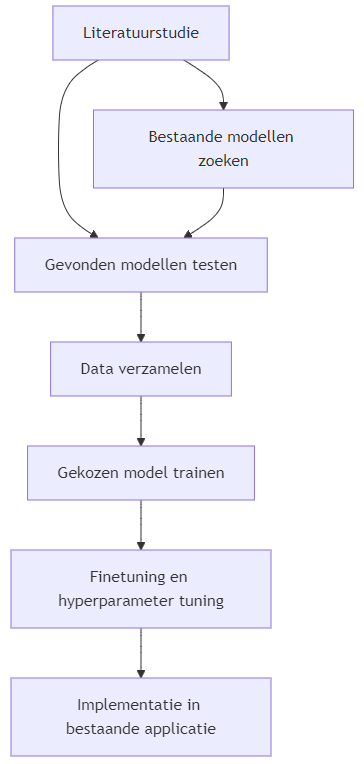
\includegraphics[scale=0.75]{./img/verloop.png}
	\caption{\label{fig:flow-chart}Voorstelling van de fasen van de bachelorproef en hun onderlinge volgorde}
\end{figure}

% Voeg hier je eigen hoofdstukken toe die de ``corpus'' van je bachelorproef
% vormen. De structuur en titels hangen af van je eigen onderzoek. Je kan bv.
% elke fase in je onderzoek in een apart hoofdstuk bespreken.

%\input{...}
%\input{...}
%...

%%=============================================================================
%% Conclusie
%%=============================================================================

\chapter{Conclusie}%
\label{ch:conclusie}

% TODO: Trek een duidelijke conclusie, in de vorm van een antwoord op de
% onderzoeksvra(a)g(en). Wat was jouw bijdrage aan het onderzoeksdomein en
% hoe biedt dit meerwaarde aan het vakgebied/doelgroep? 
% Reflecteer kritisch over het resultaat. In Engelse teksten wordt deze sectie
% ``Discussion'' genoemd. Had je deze uitkomst verwacht? Zijn er zaken die nog
% niet duidelijk zijn?
% Heeft het onderzoek geleid tot nieuwe vragen die uitnodigen tot verder 
%onderzoek?

\lipsum[76-80]



%---------- Bijlagen -----------------------------------------------------------

\appendix

\chapter{Onderzoeksvoorstel}

Het onderwerp van deze bachelorproef is gebaseerd op een onderzoeksvoorstel dat vooraf werd beoordeeld door de promotor. Dat voorstel is opgenomen in deze bijlage.


\section*{Samenvatting}

% Kopieer en plak hier de samenvatting (abstract) van je onderzoeksvoorstel.
Ondanks het feit dat de zorgsector de dag van vandaag vooral op persoonsgerichte zorgverlening focust, ervaren oudere patiënten vaak dat de communicatie te betuttelend is. Dit fenomeen staat bekend als elderspeak of secondary babytalk. Om dit tegen te gaan is er vanuit de opleiding verpleegkunde aan HOGENT het initiatief genomen om een applicatie te gebruiken die de studenten erop wijst als ze gebruik maken van elderspeak. Deze applicatie werd reeds ontworpen in voorgaande bachelorproeven, maar er ontbreken nog een aantal functionaliteiten voordat deze gebruikt kan worden in de opleiding. Deze paper heeft als doel de mogelijkheid te bieden om in de applicatie enkel de stem van de zorgverlener te analyseren en signalen van secondary babytalk op te sporen. Dit wordt bereikt aan de hand van het zoeken naar en trainen van geschikte modellen die stemmen kunnen onderscheiden. Het meest geschikte model wordt nadien geïmplementeerd in de applicatie. Het beoogde resultaat van deze paper is een volledig getraind model dat succesvol stemmen kan onderscheiden en geïntegreerd is in de applicatie.

% Verwijzing naar het bestand met de inhoud van het onderzoeksvoorstel
% TODO: 
%---------- Inleiding ---------------------------------------------------------

% TODO: Is dit voorstel gebaseerd op een paper van Research Methods die je
% vorig jaar hebt ingediend? Heb je daarbij eventueel samengewerkt met een
% andere student?
% Zo ja, haal dan de tekst hieronder uit commentaar en pas aan.

%\paragraph{Opmerking}

% Dit voorstel is gebaseerd op het onderzoeksvoorstel dat werd geschreven in het
% kader van het vak Research Methods dat ik (vorig/dit) academiejaar heb
% uitgewerkt (met medesturent VOORNAAM NAAM als mede-auteur).
% 

\section{Inleiding}%
\label{sec:inleiding}

Waarover zal je bachelorproef gaan? Introduceer het thema en zorg dat volgende zaken zeker duidelijk aanwezig zijn:

\begin{itemize}
  \item kaderen thema
  \item de doelgroep
  \item de probleemstelling en (centrale) onderzoeksvraag
  \item de onderzoeksdoelstelling
\end{itemize}

Denk er aan: een typische bachelorproef is \textit{toegepast onderzoek}, wat betekent dat je start vanuit een concrete probleemsituatie in bedrijfscontext, een \textbf{casus}. Het is belangrijk om je onderwerp goed af te bakenen: je gaat voor die \textit{ene specifieke probleemsituatie} op zoek naar een goede oplossing, op basis van de huidige kennis in het vakgebied.

De doelgroep moet ook concreet en duidelijk zijn, dus geen algemene of vaag gedefinieerde groepen zoals \emph{bedrijven}, \emph{developers}, \emph{Vlamingen}, enz. Je richt je in elk geval op it-professionals, een bachelorproef is geen populariserende tekst. Eén specifiek bedrijf (die te maken hebben met een concrete probleemsituatie) is dus beter dan \emph{bedrijven} in het algemeen.

Formuleer duidelijk de onderzoeksvraag! De begeleiders lezen nog steeds te veel voorstellen waarin we geen onderzoeksvraag terugvinden.

Schrijf ook iets over de doelstelling. Wat zie je als het concrete eindresultaat van je onderzoek, naast de uitgeschreven scriptie? Is het een proof-of-concept, een rapport met aanbevelingen, \ldots Met welk eindresultaat kan je je bachelorproef als een succes beschouwen?

%---------- Stand van zaken ---------------------------------------------------

\section{Literatuurstudie}%
\label{sec:literatuurstudie}

Hier beschrijf je de \emph{state-of-the-art} rondom je gekozen onderzoeksdomein, d.w.z.\ een inleidende, doorlopende tekst over het onderzoeksdomein van je bachelorproef. Je steunt daarbij heel sterk op de professionele \emph{vakliteratuur}, en niet zozeer op populariserende teksten voor een breed publiek. Wat is de huidige stand van zaken in dit domein, en wat zijn nog eventuele open vragen (die misschien de aanleiding waren tot je onderzoeksvraag!)?

Je mag de titel van deze sectie ook aanpassen (literatuurstudie, stand van zaken, enz.). Zijn er al gelijkaardige onderzoeken gevoerd? Wat concluderen ze? Wat is het verschil met jouw onderzoek?

Verwijs bij elke introductie van een term of bewering over het domein naar de vakliteratuur, bijvoorbeeld~\autocite{Hykes2013}! Denk zeker goed na welke werken je refereert en waarom.

Draag zorg voor correcte literatuurverwijzingen! Een bronvermelding hoort thuis \emph{binnen} de zin waar je je op die bron baseert, dus niet er buiten! Maak meteen een verwijzing als je gebruik maakt van een bron. Doe dit dus \emph{niet} aan het einde van een lange paragraaf. Baseer nooit teveel aansluitende tekst op eenzelfde bron.

Als je informatie over bronnen verzamelt in JabRef, zorg er dan voor dat alle nodige info aanwezig is om de bron terug te vinden (zoals uitvoerig besproken in de lessen Research Methods).

% Voor literatuurverwijzingen zijn er twee belangrijke commando's:
% \autocite{KEY} => (Auteur, jaartal) Gebruik dit als de naam van de auteur
%   geen onderdeel is van de zin.
% \textcite{KEY} => Auteur (jaartal)  Gebruik dit als de auteursnaam wel een
%   functie heeft in de zin (bv. ``Uit onderzoek door Doll & Hill (1954) bleek
%   ...'')

Je mag deze sectie nog verder onderverdelen in subsecties als dit de structuur van de tekst kan verduidelijken.

%---------- Methodologie ------------------------------------------------------
\section{Methodologie}%
\label{sec:methodologie}

Hier beschrijf je hoe je van plan bent het onderzoek te voeren. Welke onderzoekstechniek ga je toepassen om elk van je onderzoeksvragen te beantwoorden? Gebruik je hiervoor literatuurstudie, interviews met belanghebbenden (bv.~voor requirements-analyse), experimenten, simulaties, vergelijkende studie, risico-analyse, PoC, \ldots?

Valt je onderwerp onder één van de typische soorten bachelorproeven die besproken zijn in de lessen Research Methods (bv.\ vergelijkende studie of risico-analyse)? Zorg er dan ook voor dat we duidelijk de verschillende stappen terug vinden die we verwachten in dit soort onderzoek!

Vermijd onderzoekstechnieken die geen objectieve, meetbare resultaten kunnen opleveren. Enquêtes, bijvoorbeeld, zijn voor een bachelorproef informatica meestal \textbf{niet geschikt}. De antwoorden zijn eerder meningen dan feiten en in de praktijk blijkt het ook bijzonder moeilijk om voldoende respondenten te vinden. Studenten die een enquête willen voeren, hebben meestal ook geen goede definitie van de populatie, waardoor ook niet kan aangetoond worden dat eventuele resultaten representatief zijn.

Uit dit onderdeel moet duidelijk naar voor komen dat je bachelorproef ook technisch voldoen\-de diepgang zal bevatten. Het zou niet kloppen als een bachelorproef informatica ook door bv.\ een student marketing zou kunnen uitgevoerd worden.

Je beschrijft ook al welke tools (hardware, software, diensten, \ldots) je denkt hiervoor te gebruiken of te ontwikkelen.

Probeer ook een tijdschatting te maken. Hoe lang zal je met elke fase van je onderzoek bezig zijn en wat zijn de concrete \emph{deliverables} in elke fase?

%---------- Verwachte resultaten ----------------------------------------------
\section{Verwacht resultaat, conclusie}%
\label{sec:verwachte_resultaten}

Hier beschrijf je welke resultaten je verwacht. Als je metingen en simulaties uitvoert, kan je hier al mock-ups maken van de grafieken samen met de verwachte conclusies. Benoem zeker al je assen en de onderdelen van de grafiek die je gaat gebruiken. Dit zorgt ervoor dat je concreet weet welk soort data je moet verzamelen en hoe je die moet meten.

Wat heeft de doelgroep van je onderzoek aan het resultaat? Op welke manier zorgt jouw bachelorproef voor een meerwaarde?

Hier beschrijf je wat je verwacht uit je onderzoek, met de motivatie waarom. Het is \textbf{niet} erg indien uit je onderzoek andere resultaten en conclusies vloeien dan dat je hier beschrijft: het is dan juist interessant om te onderzoeken waarom jouw hypothesen niet overeenkomen met de resultaten.



%%---------- Andere bijlagen --------------------------------------------------
% TODO: Voeg hier eventuele andere bijlagen toe. Bv. als je deze BP voor de
% tweede keer indient, een overzicht van de verbeteringen t.o.v. het origineel.
%\input{...}

%%---------- Backmatter, referentielijst ---------------------------------------

\backmatter{}

\setlength\bibitemsep{2pt} %% Add Some space between the bibliograpy entries
\printbibliography[heading=bibintoc]

\end{document}
